\documentclass[12pt]{article}
\usepackage[utf8]{inputenc}
\usepackage{hyperref}

\title{Miscellaneous Problems}
\author{Eric Xiao}
\date{March 21, 2020}

\usepackage{natbib}
\usepackage{graphicx}
\usepackage{tikz}
\usetikzlibrary{arrows}
\usepackage{tkz-euclide}
\usepackage{textcomp}

\addtolength{\textwidth}{1.0in}
\addtolength{\textheight}{0.75in}
\addtolength{\evensidemargin}{-0.75in}
\addtolength{\oddsidemargin}{-0.75in}
\addtolength{\topmargin}{-1.0in}

\begin{document}

\maketitle

\begin{enumerate}
    \itemsep3.0em
    \item {What is the value of angle {$x$\textdegree} in this diagram?
    
        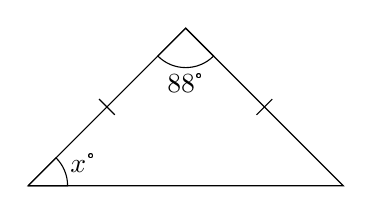
\begin{tikzpicture}
            \draw (0,0) -- (2,2) -- (4,0) -- (0,0);
            \draw (2,2) -- +(225:0.5cm) arc (225:315:0.5cm) node at (2,1.3) {88\textdegree} -- cycle;
            \draw (0,0) -- +(45:0.5cm) arc (45:0:0.5cm) node at (22.5:0.75cm) {$x$\textdegree} -- cycle;
            \draw (0.9,1.1) -- (1.1,0.9);
            \draw (2.9,0.9) -- (3.1,1.1);
        \end{tikzpicture}
    }
    
    \item {Fred's birthday was on a Monday and was exactly 37 days after Pat's birthday. Julie's birthday was 67 days before Pat's birthday. On what day of the week was Julie's birthday?}
    
    \item {What is the units digit in $7^{2020}$ when expanded?}
    
    \item {To paint a cube with edge length 3 centimeters requires 2 grams of paint. How much paint (in grams) is required to paint a cube of edge length 12 centimeters?}

    \item {If $a$, $b$, and $c$ are positive integers with $a$ x $b$ = 13, $b$ x $c$ = 52, and $a$ x $c$ = 4, what is the value of $a$ x $b$ x $c$?}
    
    \item {Alfredo, Cameron, Kasi, Hugo and Shin are to be seated around a circular table. Alfredo refuses to sit next to Cameron. How many possible different seating arrangements are there?}
    
    \item {A triangle has side lengths 6, 8, 10. A point P is chosen randomly inside the triangle. What is the probability that the distance from P to the nearest vertex is more than 2?}
    
    \item {A machine called Algo takes a number as an input and uses a procedure to convert that number into a different number, which the machine produces as output. The procedure is as follows for one conversion:
    
    \begin{enumerate}
        \item {Add 4 to the input number.}
        \item {Multiply the number in the previous step by 2.}
        \item {Take the square root of the number obtained in the previous step. If the result is not an integer, round that number $down$ to the nearest integer.}
    \end{enumerate}
    
    For instance, Algo will produce 5 as an output if the number 9 was taken as input (9 $\rightarrow$ 13 $\rightarrow$ 26 $\rightarrow$ 5).  If you let Algo run for more than one conversion, it will take the output from the previous conversion as input for the next conversion (e.g. 9 as input - first conversion: 9 $\rightarrow$ 5; second conversion: 5 $\rightarrow$ 4). If you gave Algo the number 15 as an initial input and let it run for 3 conversions, what will be its final output?}
    
    \item {The surface area of a cylinder's curved surface is 7 times larger than the surface area of one of its bases. What is the ratio of the cylinder's radius to the cylinder's height? (Write the ratio as a fraction in the form of $\frac{a}{b}$, with $a$ and $b$ in lowest terms.)}
    
    \item {What is the largest integer $n$ such that the quantity $50!$/$(5!)^n$ is an integer as well? (Note: $n!$ = $n$ x ($n-1$) x ($n-2$) x ... x $3$ x $2$ x $1$.)}

\end{enumerate}

\end{document}
